\documentclass[11pt]{article}
\usepackage[margin=1in]{geometry}
\usepackage{amsmath}
\usepackage{booktabs}
\usepackage{longtable}
\usepackage{graphicx}
\usepackage{array}
\usepackage{caption}
\usepackage{float}
\usepackage[table]{xcolor}
\usepackage{hyperref}
\hypersetup{hidelinks}
\usepackage{gensymb}
% Shared archived-soil pH constants used by the Supplementary Information.
% Numerical values are generated from immutable dataset
% EQ-PH-SHARED-v1.0.0. Manuscript prose is written directly in main.tex and
% supplement.tex; this file contains no prose-bearing commands.

% Generated by scripts/analysis/render_ph_ecology_tex.py.
% Do not edit values by hand.
\newcommand{\PHDatasetVersion}{EQ-PH-SHARED-v1.0.0}
\newcommand{\PHSourceSHA}{701db2a771b257da09bb276c8ca29df4408ba5986bd515821ccea275a8c692c1}
\newcommand{\PHSourceRows}{1168}
\newcommand{\PHDeclaredRows}{1218}
\newcommand{\PHAdmitted}{712}
\newcommand{\PHPending}{356}
\newcommand{\PHDepleted}{45}
\newcommand{\PHDateQuarantine}{36}
\newcommand{\PHColumnQuarantine}{0}
\newcommand{\PHQCQuarantine}{19}
\newcommand{\PHTotalQuarantine}{55}
\newcommand{\PHMeasurementSessions}{29}
\newcommand{\PHMatchedSpecimens}{702}
\newcommand{\PHAlphaGroups}{562}
\newcommand{\PHCompositionGroups}{558}
\newcommand{\PHTripOneGroups}{143}
\newcommand{\PHTripTwoGroups}{13}
\newcommand{\PHTripThreeGroups}{141}
\newcommand{\PHTripFourGroups}{156}
\newcommand{\PHTripFiveGroups}{109}
\newcommand{\PHMinimum}{7.29}
\newcommand{\PHMaximum}{9.98}
\newcommand{\PHMean}{7.986}
\newcommand{\PHSD}{0.240}
\newcommand{\PHAlphaEstimate}{0.185}
\newcommand{\PHAlphaCILow}{-0.332}
\newcommand{\PHAlphaCIHigh}{0.703}
\newcommand{\PHAlphaP}{0.483}
\newcommand{\PHDeepSurfaceDifference}{0.003}
\newcommand{\PHDeepSurfaceSites}{60}
\newcommand{\PHDeepSurfaceNonzeroSites}{60}
\newcommand{\PHDeepSurfaceQ}{0.763}
\newcommand{\PHRootSurfaceDifference}{-0.037}
\newcommand{\PHRootSurfaceSites}{60}
\newcommand{\PHRootSurfaceNonzeroSites}{60}
\newcommand{\PHRootSurfaceQ}{0.000534}
\newcommand{\PHRootDeepDifference}{-0.016}
\newcommand{\PHRootDeepSites}{60}
\newcommand{\PHRootDeepNonzeroSites}{59}
\newcommand{\PHRootDeepQ}{4.08\times10^{-4}}
\newcommand{\PHBrayEightyRtwo}{0.00261}
\newcommand{\PHBrayEightyP}{0.275}
\newcommand{\PHBrayNinetyFiveRtwo}{0.00256}
\newcommand{\PHBrayNinetyFiveP}{0.277}
\newcommand{\PHCLRMinimumRtwo}{0.00263}
\newcommand{\PHCLRMaximumRtwo}{0.00275}
\newcommand{\PHCLRMinimumP}{0.084}
\newcommand{\PHCLRMaximumP}{0.280}
\newcommand{\PHPrimaryCLRRtwo}{0.00274}
\newcommand{\PHPrimaryCLRP}{0.126}
\newcommand{\PHGeographyBeforeRtwo}{0.358}
\newcommand{\PHGeographyAfterRtwo}{0.196}
\newcommand{\PHGeographyP}{0.001}
\newcommand{\PHGeographySites}{60}
\newcommand{\PHGeographyResidualDf}{57}
\newcommand{\PHGeographyAttenuation}{45.3}
\newcommand{\PHSpatialRtwo}{0.846}
\newcommand{\PHSpatialP}{0.001}
\newcommand{\PHMaximumGroupTrip}{4}
\newcommand{\PHMaximumGroupSite}{60}
\newcommand{\PHMaximumGroupPosition}{Rhizosphere}
\newcommand{\PHMaximumGroupSpecimens}{1}
\newcommand{\PHExcludeMaximumSpatialRtwo}{0.826}
\newcommand{\PHExcludeMaximumSpatialP}{0.001}
\newcommand{\PHExcludeMaximumGeographyRtwo}{0.187}
\newcommand{\PHExcludeMaximumSiteSpatialRtwo}{0.833}
\newcommand{\PHExcludeMaximumSiteGeographyRtwo}{0.188}
\newcommand{\PHCompleteTripSiteBlocks}{144}
\newcommand{\PHCompleteSites}{60}
\newcommand{\PHFriedmanChiSquare}{19.757}
\newcommand{\PHFriedmanP}{5.13\times10^{-5}}


\renewcommand{\thesection}{S\arabic{section}}
\renewcommand{\thetable}{S\arabic{table}}
\renewcommand{\thefigure}{S\arabic{figure}}
\newcolumntype{P}[1]{>{\raggedright\arraybackslash}p{#1}}

\title{Supplementary Information\\
\large Landscape-scale bacterial biogeography across the Rub' al-Khali
reveals recurring spatial and soil-position structure}
\author{}
\date{}

\begin{document}
\maketitle

\section{Analysis provenance}

The grouped ecology, rainfall, spatial, XRF, network and encoded-function
modules reported in the manuscript write machine-readable TSV and JSON results
under \path{analysis/v3} and \path{analysis/xrf_audit}. Input manifests,
parameter files and checksums are present only for the modules that emit them.
Seeds were $20260723$ for the core paired, XRF-rescue,
spatial-turnover, phylogenetic and functional-redundancy analyses; $20260725$
for compartment composition, depth/extraction and XRF CLR; and $20260728$ for
geographic prediction, spatial-resolution and distance-decay analyses.
The post-hoc rainfall pulse analysis used seed $20260804$ and $19{,}999$
conditional lag rotations for each model. Its search covered $60$ candidate
peak times and three diversity endpoints. Sampling and peak-selection
intervals used $9{,}999$ whole-site bootstrap samples with seed $20260805$.
The cross-desert context analysis used seed $20260804$, $9{,}999$ depth-zone
label permutations and $100$ rarefactions per Atacama pit profile.
The site-level climate analysis declares separate Benjamini--Hochberg families
for nine diversity and $600$ genus tests. Its diversity intervals used
$9{,}999$ paired-site bootstrap samples with seed $20260805$. The PICRUSt2
ecology analysis used seed $20260804$, $9{,}999$ whole-site permutations and
$2{,}000$ site bootstraps; its three primary pathway-profile contrasts, $600$
paired pathway tests and $200$ geographic pathway tests form separate declared
families.
The spatial and distance-decay modules use delete-one-site jackknife intervals;
every pair involving the omitted site is removed in pairwise analyses.
The archived-soil pH module uses dataset version \PHDatasetVersion,
$999$ permutations with seed $20260802$, an exact input manifest, recorded
software versions and output checksums under
\path{analysis/v3/ph_shared_v1/}.
The primary paired and evenness tables use the same $1{,}000{,}000$-resample
bootstrap implementation and seed $20260723$; their estimates, intervals and
unadjusted $p$ values for the identical Shannon estimand agree. Their $q$
values need not agree because the primary Shannon family contains three
all-campaign plus $14$ campaign-specific contrasts, whereas the evenness module
corrects three all-campaign contrasts. Printed Shannon intervals come from
\path{analysis/v3/results/paired_compartment_effects.tsv}; the evenness rerun
must reproduce them. Multiplicity correction was applied within each declared
family, not as one omnibus correction across the distinct diversity,
composition, rainfall and XRF analyses. The network parameter file records its
base and phase seeds. PMA mean-difference intervals used $99{,}999$
paired-aliquot bootstrap samples and encoded-function agreement used $9{,}999$
whole-site bootstrap samples, both with seed $20260805$. A typed summary of
$44$ headline
estimates, methods and source results is archived under
\path{analysis/v3/headline_uncertainty/}.
Table~\ref{tab:denominators-revised}
distinguishes the observational units and cohorts used by each analysis.

\section{Data layers and denominator reconciliation}

\begingroup
\footnotesize
\begin{longtable}{P{4.2cm}P{2.5cm}P{5.9cm}}
\caption{Current analysis denominators. Different denominators correspond to
different data products, not interchangeable estimates.}
\label{tab:denominators-revised}\\
\toprule
Data product & $n$ & Analytical role \\
\midrule
\endfirsthead
\multicolumn{3}{l}{\tablename\ \thetable\ continued}\\[2pt]
\toprule
Data product & $n$ & Analytical role \\
\midrule
\endhead
\midrule
\multicolumn{3}{r}{Continued on the next page}\\
\endfoot
\bottomrule
\endlastfoot
Observed ecology site labels & $64$ & Numeric site labels represented in the
alpha table \\
Primary repeated-site cohort & $60$ sites; $1{,}227$ profiles & Sites $1--60$,
aggregated to $633$ site--campaign--position observations \\
QC-passed alpha-diversity profiles & $1{,}237$ & Biological profiles with at
least $1{,}000$ reads; $1{,}227$ profiles belong to the $60$-site repeated-inference
cohort \\
Canonical all-trip feature table & $1{,}271$ & Biological and control profiles;
source for the $351{,}472$-ASV feature universe \\
Complete field-XRF sessions & $71$ of $106$ log entries & Trip~$5$ in-situ handheld
measurements retained at $58$ sites from a log spanning $59$ sites; the log links
TestID to site but not to a physical aliquot or compartment \\
Laboratory-XRF analytical records & $725$ & $547$ records from Trips~$1--4$ plus
$178$ Trip~$5$ records; all included in the canonical elemental-axis analysis \\
Laboratory-XRF/alpha joins & $622$ & Site--campaign--compartment observations on
the $60$ core sites \\
Laboratory-XRF/composition joins & $621$ & Bray--Curtis community analysis after
minimum-count filtering \\
Archived-soil pH/ecology joins & $\PHAlphaGroups$ alpha;
$\PHCompositionGroups$ composition & Quality-controlled, incomplete
shared archived-sample pH cohort (\PHDatasetVersion) \\
Matched network cohort & $170$ per compartment & Same campaign--site groups in
surface, shallow subsurface and root-adjacent soil; $60$ sites \\
Resolution-matched encoded-function null & $150$ & $27$ surface, $44$ shallow
subsurface and $79$ root-adjacent profiles; $990$ annotated genomes, $2{,}000$
retained KOs and $28.5\,\%$ mean annotated-catalog fraction \\
PICRUSt2--shotgun overlap & $125$ & Whole-KO-profile comparison \\
PICRUSt2 ecology cohort & $1{,}227$ profiles; $633$ grouped profiles & Sixty core
sites, $462$ predicted MetaCyc pathways and $172$ complete three-position
site--campaign blocks \\
Retained CBB-marker genome records & $132$ & RuBisCO plus
phosphoribulokinase annotations; the complete upstream screened-genome
manifest was not preserved, so no denominator or fraction is reported \\
Rainfall pulse cohort & $617$ site--campaign--position groups & Technical means
for $196$ surface, $203$ shallow-subsurface and $218$ root-adjacent groups across $60$
sites; the paired bulk-soil sensitivity used $179$ pairs; $20$ distinct NASA POWER
daily precipitation series \\
PMA pairs & $9$ & Trip~$5$ treated-versus-untreated aliquots \\
\end{longtable}
\endgroup

The PMA ASV count table, $150$ CoverM profiles and eggNOG-derived annotations
used by the downstream analyses are enumerated with paths and checksums in the
analysis manifests under \path{analysis/v3/}. Reproducing the upstream PMA and
shotgun processing additionally requires the corresponding raw-read
accessions, dereplicated MAG FASTAs and processing metadata.

The final canonical \texttt{feature-table-trips1-5.tsv} comprised $1{,}271$
profiles and $351{,}472$ ASVs. The ecological dataset excluded $24$ extraction-blank
profiles and ten biological profiles with fewer than $1{,}000$ reads, leaving
$1{,}237$ quality-controlled biological profiles. Of these, $1{,}227$ profiles from
sites $1--60$ formed the repeated-inference cohort. Ten profiles from four
Trip~$1$-only locations were retained for description but not repeated-site
inference. The primary ecological analysis applied no rare-feature or
contaminant filter. Hurlbert expected richness was standardized at $25{,}000$ reads.
Sixty of the $1{,}237$ profiles, including $55$ of the $1{,}227$ core profiles, fell
below that depth, leaving $1{,}177$ full-cohort and $1{,}172$ core expected-richness
values. Shannon diversity remained available at full depth for every profile.

\subsection{Wet-laboratory and amplicon-processing record}

Each field replicate was placed in a sterile tube by scooping directly with
the tube or with a sterile plastic spoon. Samples were held at
$-20\,^{\circ}\mathrm{C}$ in an Engel MR040F portable freezer during each
expedition and transferred to $-80\,^{\circ}\mathrm{C}$ in the laboratory.
DNA extraction used $0.9$--$1.2\,\mathrm{g}$ of soil, the QIAGEN PowerLyzer
PowerSoil kit (catalogue \texttt{12855-50}) or DNeasy PowerSoil Pro kit
(catalogue \texttt{47014}), PowerLyzer~$24$ homogenization, manual or QIACube
Connect processing, and a $50\,\mu\mathrm{L}$ elution.

The Bakt\_341F and Bakt\_785R primers carried Illumina overhang adapters.
Primary amplification used the QIAGEN Multiplex PCR Kit (catalogue
\texttt{206143}): $95\,^{\circ}\mathrm{C}$ for $15\,\mathrm{min}$; $35$
cycles of $94\,^{\circ}\mathrm{C}$ for $30\,\mathrm{s}$,
$57\,^{\circ}\mathrm{C}$ for $90\,\mathrm{s}$ and
$72\,^{\circ}\mathrm{C}$ for $90\,\mathrm{s}$; and a final
$72\,^{\circ}\mathrm{C}$ extension for $10\,\mathrm{min}$. Amplicons were
checked on a $2\,\%$ agarose gel, indexed and cleaned following the Illumina
$16$S library protocol, quantified with the Qubit high-sensitivity
double-stranded DNA assay, sized on an Agilent TapeStation~$4200$, pooled by
concentration and size, and sequenced as paired $2\times250$-base reads on a
NovaSeq~$6000$.

The canonical feature table was generated with version v2.14.0 of the nf-core
Ampliseq workflow. It used DADA2 and SILVA~$138.2$. The exact command, resource configuration and portable
samplesheet are in \path{data/processed/amplicon/}. The retained laboratory
record does not specify the PCR template input mass, exact index-kit and
adapter part numbers, cleanup and indexing cycle counts, NovaSeq reagent kit,
or container digest. These items remain unknown rather than inferred.

\subsection{Assay-aware control analysis}

The $24$ control profiles in the canonical table comprise \texttt{EB1}--\texttt{EB18}
and \texttt{Negative1}, \texttt{Negative2}, and
\texttt{Negative4}--\texttt{Negative7}; all were extraction blanks. One blank
was processed per extraction day, and an
extraction day could include samples from several field trips. A trip value is
therefore not applicable to an extraction blank. The extraction-day workbook
maps EB1--EB17 to dates and $220$ Trip~$5$ biological profiles, of which $217$ occur
in the canonical table. These links do not assign an EB exclusively to a trip.
EB18 and the six \texttt{Negative}-labelled profiles
lack extraction-day mappings and were retained for characterization only.

The primary screen pooled EB1--EB17 because there was only one blank per
extraction batch. It used an uncorrected one-sided Fisher $p<0.1$ and required
presence in at least two blanks. Positive controls were excluded from
training. The screen identified $351$ of $351{,}472$ ASVs; at the same threshold,
relaxing the minimum to one blank called $12{,}051$ ASVs. Those ASVs were
removed only from the $217$ biological profiles linked to the mapped Trip~$5$
batches; the other $1{,}020$ ecological profiles were unchanged, and the
unfiltered canonical table was retained. Removal accounted for $2.1866\,\%$ of
reads across the mapped profiles, with median $0.4027\,\%$ and maximum
$56.5951\,\%$ per profile. No profile fell below $25{,}000$ reads. Shannon diversity
before and after filtering had Spearman $\rho=0.99496$ (median change
$-0.00340$; maximum absolute change $0.67805$), and raw richness had
$\rho=0.99995$ (median change $-11$ ASVs; maximum absolute change $81$).
All $25$ tracked headline metrics retained their scientific verdicts. Frequency
modelling was not run because control DNA concentrations were unavailable.

The positive-control design was trip-specific. Trips~$1$ and $2$ used purified-DNA
ZymoBIOMICS HMW DNA Standard D6322, which can evaluate PCR, library and
sequencing performance but not extraction or lysis. Trip~$3$ used whole-cell
ZymoBIOMICS Microbial Community Standard D6300 and therefore included
extraction. Trip~$4$ had no positive control. Trip~$5$ also used D6300, but its
positive and negative control pair was sequenced by shotgun metagenomics rather
than $16$S. Seven unambiguously positive-labelled profiles in the
pre-decontamination $16$S table were used only for evaluation. At genus level,
the two Trip~$1$ profiles recovered three and two of seven expected bacterial
genera; the two Trip~$2$ profiles recovered seven and zero; and the three Trip~$3$
profiles recovered one, eight and eight of eight. Manufacturer genomic-DNA
fractions were not interpreted as expected $16$S read fractions. Under the
trip-design product hypotheses, the fractions of all reads assigned to
expected bacterial genera were $5.85$, $12.33$, $31.05$, $0$, $0.05$, $100$ and
$99.99\,\%$ for \texttt{e0553\_Ctrl\_2}, \texttt{e0554\_Ctrl\_3},
\texttt{e0872\_TMC1}, \texttt{e0874\_Positive},
\texttt{e8294\_FPosCtrl1}, \texttt{e8661\_FPosCtrl2} and
\texttt{e8665\_FPosCtrl3}, respectively. Only the last two met the declared
descriptive mock-dominated threshold of at least $95\,\%$. These
library-to-product assignments remain provisional; recovery does not confirm
their identities. Exact
mock-associated ASVs were also traced into negative controls, neighbouring
indices and biological profiles, but overlap alone cannot distinguish natural
occurrence, cross-contamination, index hopping or a mislabelled source
library. The metadata-negative profile
\texttt{e0323\_Ctrl\_1\_Trip1} was not promoted to a positive control from its
name.

The audit follows the principle that all available processing controls should
be sequenced and reported, with positive controls reserved for evaluating
expected recovery rather than training a contaminant filter
\cite{fierer2025controls}. Three paired $16$S libraries with explicit PCR or NTC
labels (\path{e0555_PCR_Ctrl_Trip1}, \path{e0875_NTC_2} and
\path{e8667_PCRCtrl}) and one Trip~$4$ workbook record already bear PCR-blank
roles in the control registry. The remaining PCR-control task is a resolvable
laboratory-metadata follow-up: confirm any additional reused or generic labels,
their reaction or batch identifiers and the biological libraries amplified in
the same batches. Until laboratory evidence confirms those links, PCR blanks remain separate from
extraction blanks and cannot support a batch-linked PCR prevalence analysis.
The material limits are that the Trip~$4$ blank covering a three-day extraction
was not sequenced, affecting all or part of $23$ sites; Trip~$5$ has no positive
control in the $16$S assay; and no sterile-bag inventory was recovered.

\subsection{Two XRF measurement workflows}

Table~\ref{tab:xrf-workflows} separates the coverage, material and analytical
use of the field and laboratory workflows.

\begin{table}[H]\centering\small
\caption{Field and laboratory XRF are distinct measurement workflows.}
\label{tab:xrf-workflows}
\begin{tabular}{P{2.4cm}P{2.8cm}P{2.6cm}P{5.5cm}}
\toprule
Workflow & Coverage & Material & Analytical use \\
\midrule
Field XRF & Trip~$5$ only; $106$ log entries across $59$ sites, of which $71$ complete
sessions at $58$ sites were retained & In situ Vanta handheld
sessions; TestID--site provenance only & Field-scale context and descriptive
Trip~$5$ site-level diagnostic; not an aliquot match, interchangeability test or
all-trip covariate \\
Laboratory XRF & All five trips; $725$ records; $622$ alpha and $621$ composition
joins & Archived collected samples measured in the laboratory &
Within-campaign elemental PCA and adjusted ecology models; Trip~$5$ settings
encoded, Trips~$1--4$ method/mode and combined-source units/LOD semantics absent \\
\bottomrule
\end{tabular}
\end{table}

The source-specific analytical tables reproduce $547$ Trips~$1--4$ records and
$178$ Trip~$5$ records. The canonical analysis includes all $725$, keeps field XRF
separate, excludes Trip-1-only sites $61--64$ from repeated-campaign inference
and reduces between-campaign location differences by standardizing elements
within campaign. This does not remove every campaign-specific variance or
method effect. Method, mode, material and diameter are encoded for Trip~$5$
laboratory records but absent from the consolidated Trips~$1--4$ source;
concentration units, limits of detection and non-detect semantics are not
machine-readable across the combined source. The Trip~$5$ field--laboratory
comparison is a site-level diagnostic because the field log contains no
physical-aliquot identifier, and it does not establish interchangeability.
Trips~$1--4$ used the maximum positive analyte repeat and Trip~$5$ retained the
last repeat. A primary-status sensitivity for the $11$ affected Trip~$5$ analytes
gave Spearman $\rho\geq0.994$, so this bookkeeping difference did not reorder
the analysis materially.

Instrument zeros were not treated as measured absence. Eleven elements
detected in at least $75\,\%$ of laboratory specimens (Al, Ca, Cl, Fe, K, Mg,
Na, P, S, Si and Ti) were transformed as $\log(1+x)$, standardized within
campaign and submitted to PCA. PC1 explained $39.2\,\%$ of variance; its largest
positive loadings were Ca ($0.413$), Mg ($0.406$), Na ($0.370$), S ($0.354$) and Cl
($0.338$), with Si negative ($-0.273$). PC1 correlated $r=0.825$ with an
internal evaporite-element reference and $r=0.976$ with the globally
standardized sensitivity axis.

The composition of the axis supports the descriptive term
\emph{evaporite-associated elemental axis}. In the site-fixed alpha model
($n=622$), the Shannon coefficient was $0.00027$ ($95\,\%$ CI
[$-0.040$,$0.041$], $p=0.990$), so no diversity association was detected. In
the primary Bray--Curtis model ($n=621$), $38$ PCoA axes retained $80.0\,\%$ of
variation and the elemental term had partial $R^{2}=0.00345$ ($p=0.056$, $999$
within-site permutations); retaining $95.0\,\%$ of variation gave a similar
$R^{2}=0.00330$ but $p=0.044$. The estimated effect size was therefore stable
across that threshold while the permutation $p$ value was not.

Because amplicon composition is compositional, a prespecified Aitchison
sensitivity reused the same $621$ joins and the unchanged axis. Genera present
in at least $20\,\%$ of groups were ranked by mean relative abundance, and the
nine combinations of $80$, $200$ or all $383$ eligible genera with a $0.5$ or $1.0$
pseudocount or multiplicative zero replacement at $0.65$ all supported the axis
after campaign, compartment and site adjustment (partial
$R^{2}=0.00311$--$0.00543$, $p=0.002$--$0.015$; primary $R^{2}=0.00358$,
$p=0.010$). The primary configuration used the top $200$ genera and a $0.5$
pseudocount. The warranted conclusion is a small conditional composition
association, identified within sites, rather than no association or an
ecologically important one. A separate diagnostic that omitted site
indicators, because they force site-mean residuals to zero, found that
site-mean CLR residuals remained spatially autocorrelated after campaign,
compartment and elemental-axis adjustment (multivariate Moran's $I=0.304$,
$p=0.001$), so the axis does not fully account for the broad geographic pattern.

XRF measures total elemental composition, not soluble salts or osmotic
stress. A same-matrix ``salinity index'' is not independent validation.
Because the analysed cohort has no independent EC measurement, we use
``evaporite-associated elemental axis'' rather than ``salinity proxy'' and make
no physiological salinity inference.

\section{Archived-soil pH sensitivity}
\label{sec:ecology-ph}

The analysis used archived-soil pH dataset version \PHDatasetVersion. We
measured pH in $767$ specimens and retained $712$ measurements with an unambiguous
measurement date, a value in the physical range, recorded calibration, an
electrode slope of $95--102\,\%$, and a pH $10$ buffer read-back of $9.9--10.1$.
$36$ measurements had ambiguous dates and $19$ did not meet session
quality-control criteria. Missing and excluded measurements were not imputed.
Coverage was incomplete and non-random, especially in campaigns $1$ and $3$
(Table~\ref{tab:ecology-ph-coverage}).

\begin{table}[H]\centering\small
\caption{Coverage and quality control of the archived-soil pH measurements.}
\label{tab:ecology-ph-coverage}
\begin{tabular}{lrrrrr}
\toprule
Campaign & Target specimens & Measured & Passed QC & Not measured & Excluded \\
\midrule
$1$ & $330$ & $157$ & $157$ & $173$ & $0$ \\
$2$ & $27$ & $23$ & $23$ & $4$ & $0$ \\
$3$ & $450$ & $192$ & $156$ & $258$ & $36$ \\
$4$ & $177$ & $175$ & $156$ & $2$ & $19$ \\
$5$ & $234$ & $220$ & $220$ & $14$ & $0$ \\
\bottomrule
\end{tabular}
\end{table}

The versioned SIO graph models each retained measurement as an existing
specimen, a PATO acidity quality (PATO:0001842), a value typed as both an SIO
measurement value (SIO:000070) and pH (SIO:001089), and an SIO measuring
process (SIO:001054). Values use the pH unit (UO:0000196); process, value,
quality, protocol, device and session links follow the same directions as the
XRF and DNA measurement patterns. Stable IRIs depend on specimen, date and
protocol rather than workbook hash. The shared version contains $\PHAdmitted$
process--quality--value sets and $\PHMeasurementSessions$ reconstructed session
groupings based on trip, date, slope and pH-10 read-back. The source workbook
does not contain a session identifier. A deposited shape map enumerates every
validated process, value, quality, protocol, device and session; a deposited
negative fixture without the pH unit is rejected. Graph-equivalent Turtle and
RDF/XML serializations are imported by the canonical knowledge graph.

The ecology join contained $\PHMatchedSpecimens$ specimens,
$\PHAlphaGroups$ alpha-diversity groups and $\PHCompositionGroups$ composition
groups across all $60$ core sites. Table~\ref{tab:ecology-ph-models} reports the
model results. Availability is non-random, especially within campaigns $1$ and
$3$, so inference is bounded to this subset.

\begin{table}[H]\centering\small
\caption{Archived-soil pH sensitivity results for \PHDatasetVersion.}
\label{tab:ecology-ph-models}
\begin{tabular}{P{5.2cm}rrrP{3.1cm}}
\toprule
Endpoint & $n$ & Effect size & $p$ & Boundary \\
\midrule
Site-fixed Shannon & $\PHAlphaGroups$ & $\beta=\PHAlphaEstimate$ & $\PHAlphaP$ & No detected diversity association \\
Primary top-$200$ CLR composition & $\PHCompositionGroups$ & partial $R^2=\PHPrimaryCLRRtwo$ & $\PHPrimaryCLRP$ & No detected direct association \\
Bray--Curtis composition, $80\,\%$ axes & $\PHCompositionGroups$ & partial $R^2=\PHBrayEightyRtwo$ & $\PHBrayEightyP$ & No detected direct association \\
Transect, same cohort before pH & $\PHGeographySites$ sites & partial $R^2=\PHGeographyBeforeRtwo$ & $\leq\PHGeographyP$ & $\PHGeographyResidualDf$ residual df; same-cohort reference \\
Transect, same cohort after pH & $\PHGeographySites$ sites & partial $R^2=\PHGeographyAfterRtwo$ & $\leq\PHGeographyP$ & $\PHGeographyResidualDf$ residual df; attenuated \\
pH trend along transect & $\PHGeographySites$ sites & partial $R^2=\PHSpatialRtwo$ & $\leq\PHSpatialP$ & $\PHGeographyResidualDf$ residual df; archived subset \\
\bottomrule
\end{tabular}
\end{table}

The pH maximum was the \PHMaximumGroupPosition\ group from campaign
$\PHMaximumGroupTrip$, site $\PHMaximumGroupSite$, based on
$\PHMaximumGroupSpecimens$ specimen. Excluding that group changed the pH
transect partial $R^2$ from $\PHSpatialRtwo$ to
$\PHExcludeMaximumSpatialRtwo$ and the pH-adjusted composition statistic from
$\PHGeographyAfterRtwo$ to $\PHExcludeMaximumGeographyRtwo$. Excluding all of
site $\PHMaximumGroupSite$ gave corresponding values of
$\PHExcludeMaximumSiteSpatialRtwo$ and
$\PHExcludeMaximumSiteGeographyRtwo$; all refit permutation tests remained at
$p\leq0.001$. The maximum therefore influences the descriptive pH gradient but
does not determine the paper's bounded conclusion.

Across $\PHCompleteSites$ sites with all $3$ positions, the pH-position
omnibus gave $\chi^2=\PHFriedmanChiSquare$ ($p=\PHFriedmanP$). The Wilcoxon
contrasts used $\PHDeepSurfaceNonzeroSites/\PHDeepSurfaceSites$,
$\PHRootSurfaceNonzeroSites/\PHRootSurfaceSites$ and
$\PHRootDeepNonzeroSites/\PHRootDeepSites$ nonzero/site differences for
shallow-subsurface--surface, root-adjacent--surface and
root-adjacent--shallow-subsurface, respectively. The differences are small;
the $\pm0.1$ pH-10 read-back quality-control band is a session
quality-control
criterion, not an estimate of soil-pH analytical resolution.

\section{Evidence status and claim boundaries}

Table~\ref{tab:claims} links each central result to its permissible
interpretation and unresolved boundary.

{\footnotesize
\begin{longtable}{P{3.0cm}P{5.0cm}P{6.0cm}}
\caption{Claim ledger for the evidence-bounded manuscript.}\label{tab:claims}\\
\toprule
Topic & Evidence & Permissible interpretation \\
\midrule
\endfirsthead
\toprule
Topic & Evidence & Permissible interpretation \\
\midrule
\endhead
Soil-position composition & $170$ complete campaign--site blocks; omnibus
pseudo-$F=17.28$, $p=0.001$; pairwise-complete cohorts of $183$, $182$ and $191$
blocks gave three CLR displacements with $p=q=0.001$; surface-to-root-adjacent
dispersion increased, but the final shallow-to-root step had $q=0.061$ &
Centroid location and spread differ among operational positions; no
plant-filter mechanism \\
Root proximity & Campaign-averaged, site-paired Shannon:
root-adjacent--surface mean $-0.130$ [$95\,\%$ CI $-0.321$, $0.079$],
$q=0.0256$; root-adjacent--shallow mean $-0.206$ [$-0.398$, $-0.001$],
$q=0.0256$, with the bootstrap upper endpoint adjacent to zero;
post-hoc normalized-evenness contrasts $-0.0315$ and
$-0.0440$, expected-richness contrasts not supported & Lower root-adjacent
Shannon accompanies lower normalized evenness; no plant-filter mechanism \\
Geography & Centred-CLR joint linear-plus-quadratic transect model partial $R^2=0.4016$,
$p=0.001$; campaign-plus-block holdout $R^2=-0.0015$; collection-order
$|\rho|=0.994$--$1.000$; residual Moran's $I$ depends on $k$ &
Repeatable transect structure without cross-campaign transport or geographic,
or dispersal attribution; the shared pH cohort below accounts for part, but
not all, of a same-cohort statistic \\
Archived-soil pH & $\PHMatchedSpecimens$ exact specimen joins;
$\PHCompositionGroups$ composition groups; direct primary CLR partial
$R^2=\PHPrimaryCLRRtwo$, $p=\PHPrimaryCLRP$; same-cohort transect partial
$R^2$ changed from $\PHGeographyBeforeRtwo$ to $\PHGeographyAfterRtwo$ after
pH adjustment & pH is a measured correlate of part of the spatial pattern;
no stable direct composition association, complete-survey estimate or causal
mediation claim \\
Assembly & Top-800-ASV laboratory-XRF elemental-axis niche diagnostic:
overall Mantel $r=-0.0837$ and closest-$30\,\%$ pairwise
$r=0.0262$; no positive short-distance phylogenetic signal &
No $\beta$NTI/RC-Bray process percentage is reported \\
Elemental axis & Within-campaign PC1 explains $39.2\,\%$; adjusted Shannon
$p=0.990$; primary CLR composition partial $R^{2}=0.00358$, $p=0.010$;
all nine CLR configurations span $0.31--0.54\,\%$ & Descriptive
evaporite-associated elemental gradient; a small conditional composition
association that does not fully account for broad geographic structure; no
salinity inference \\
Long-term climate & Forty-nine months at each of $60$ sites; all nine
temperature/rain/humidity associations with Shannon, expected richness and
evenness pass global correction; $111--112$ of $200$ genus tests per climate
summary pass a $600$-test correction & Climate gradients coincide with bacterial
diversity and abundance gradients; their close covariation with the transect
prevents separate causal attribution \\
Campaign/depth & Campaign-by-position Wald $p=0.00831$ unadjusted and
$p=0.17476$ after log-sequencing-depth adjustment; kit recorded for
$858$/$1{,}237$ profiles; QIACube occurs only in campaigns $4$ and $5$, whereas
campaigns $1--3$ contain multiple recorded kits &
Campaign-by-position interaction is depth-sensitive; extraction fits do not
remove laboratory batch effects; no season or persistent-refugium claim \\
Rain response & Rise-and-decay model across $617$ site--campaign--position
groups, $60$ candidate peaks and $3$ endpoints; $19{,}999$ conditional lag
rotations; expected richness peaked at $2$ days with NASA POWER
($p=0.0560$) and at $1$ day with Open-Meteo ($p=0.0432$) after directional
family-wise correction & Bounded evidence for a short richness association
during the first several days; no causal or exact-latency claim \\
PMA & $9$ Trip~$5$ pairs; Hurlbert expected richness lower after treatment, no Shannon
difference detected & Direct paired endpoints only; no quantitative relic
fraction or survey-wide generalization \\
Contamination & Assay-aware screen: $17$ extraction-day blanks with batch links
to Trip~$5$ profiles;
$351$/$351{,}472$ candidate ASVs; $2.19\,\%$ of reads removed across $217$ mapped
profiles; seven $16$S positive profiles evaluated; $25$ headline metrics rerun &
All headline verdicts stable under the bounded filter; complete PCR-blank
batch mapping awaits laboratory confirmation, while the absent Trip~$4$ positive
and Trip~$5$ $16$S positive and one unsequenced Trip~$4$ blank bound interpretation \\
Conditional networks & $170$ matched observations per compartment; $80$ genera;
CLR Graphical Lasso; $200$ site-cluster bootstraps; null/raw edge ratio $0.05374$
& Stable null-calibrated conditional associations occur within each
compartment, but comparative density ordering is not stable; no interaction,
hub, complexity, resilience or campaign/season claim \\
Encoded-functional turnover & $150$ analysis-ready metagenome profiles; $990$ annotated genomes; $2{,}000$
KOs; observed $0.13386$ versus taxonomic $0.82272$ and null median $0.08733$,
lower-tail $p=1.0$, upper-tail $p=0.001$ & Lower raw encoded-functional than
taxonomic turnover, but higher than the resolution-matched genome-label null;
no convergence, redundancy or mechanism claim \\
PICRUSt2 & $1{,}227$ core profiles; pathway-composition transect $R^2=0.234$,
$p=0.0001$; $172$ complete position blocks; $125$ shotgun matches with whole-KO
median $\rho=0.74$; RuBisCO $r=0.16$, $p=0.067$ & Broad predicted potential
follows geography and soil position and agrees with shotgun at whole-profile
scale; no measured activity or rare-marker validation \\
Carbon markers & $132$ genome records with RuBisCO+PRK annotations; complete upstream
screened-genome denominator unavailable & Candidate Calvin-cycle genomic
potential, not a genome fraction or activity \\
Trace-gas markers & Product/KO annotation screen without catalytic,
phylogenetic, synteny or direct-read confirmation & No pathway-identity or
activity claim \\
\bottomrule
\end{longtable}
}

\section{Compartment and spatial evidence}

\subsection{Paired compartment composition}

The primary composition analysis aggregated genus counts within
campaign--site--position and retained $170$ complete three-position blocks
across $60$ sites for the omnibus test. Genera present in at least $20\,\%$ of groups were ranked by
mean relative abundance; the primary configuration used the leading $200$
genera, a $0.5$ pseudocount and centred-log-ratio (CLR) coordinates. Permuting
position labels within blocks gave an omnibus pseudo-$F=17.2797$ with
$p=0.001$.

Pairwise location tests used their respective pairwise-complete cohorts and
sign-flipped the mean within-block CLR difference vector across sites.
Standardized displacements were $0.3312$ for shallow subsurface minus surface
($n=183$ blocks), $0.4328$ for root-adjacent minus surface ($n=182$) and $0.4780$
for root-adjacent minus shallow subsurface ($n=191$); each had permutation $p=0.001$
and Benjamini--Hochberg $q=0.001$. The directions and location results
persisted with $80$, $200$ or all $384$ eligible genera, three zero treatments and
each leave-one-campaign refit. Because the test targets the paired mean
difference vector, it is exact under the paired-symmetry null even when
within-position dispersion differs.

Dispersion increased monotonically from surface to shallow subsurface to
root-adjacent soil. The shallow-subsurface--surface difference was $1.3776$
(bootstrap $95\,\%$ CI [$0.4411$,$2.3748$], permutation $q=0.015$);
root-adjacent--surface was $2.3866$ ([$1.5502$,$3.2123$], $q=0.003$); and
root-adjacent--shallow subsurface was $1.0090$ ([$0.0556$,$2.0550$], $q=0.061$).
The last permutation contrast does not pass $q<0.05$, despite its bootstrap
interval. The composition result describes the operational collection
position and does not establish a plant selective filter.

\subsection{Alpha diversity and post-hoc normalized evenness}

For all-campaign paired contrasts, profiles were averaged within
site--campaign--position and then across campaigns within site and position.
Among $60$ sites, root-adjacent minus surface Shannon diversity had mean
$-0.130$ (median $-0.250$, bootstrap $95\,\%$ CI [$-0.321$,$0.079$],
Wilcoxon $q=0.0256$). Root-adjacent minus shallow subsurface had mean
$-0.206$ (median $-0.430$, $95\,\%$ bootstrap CI
[$-0.398$,$-0.001$], upper endpoint adjacent to zero, $q=0.0256$).
The endpoint's sign is not used as evidence; the distributional claim is
carried by the paired Wilcoxon result. Shallow subsurface minus surface had
mean $0.075$ ($95\,\%$ CI
[$-0.089$,$0.235$], $q=0.189$).

A post-hoc decomposition used
$H/\log(E[S_{25k}])$, where $E[S_{25k}]$ is Hurlbert expected richness at
$25{,}000$ reads. This is a normalized-evenness sensitivity, not conventional
Pielou evenness. Root-adjacent minus surface normalized evenness was
$-0.03148$ ($95\,\%$ CI [$-0.04477$,$-0.01863$],
$q=2.76\times10^{-6}$), root-adjacent minus shallow subsurface was
$-0.04398$ ([$-0.05717$,$-0.03131$], $q=2.13\times10^{-7}$), and shallow
subsurface minus surface was $+0.01250$ ([$0.00084$,$0.02508$], $q=0.0121$).
Campaign- and log-depth-adjusted GEE contrasts retained these directions:
$-0.02841$ ($p=1.67\times10^{-5}$), $-0.04260$
($p=3.24\times10^{-11}$) and $+0.01419$ ($p=0.0125$), respectively.
Expected-richness contrasts did not pass their three-test correction
($q=0.814$, $0.0878$ and $0.0675$ for root-adjacent--surface,
root-adjacent--shallow and shallow--surface). Hurlbert richness was unavailable
for $55$ core profiles below $25{,}000$ reads, and normalized evenness was also
undefined for one single-ASV profile; its GEE used $617$ of $633$ blocks.

\subsection{Transect structure, transport and spatial resolution}

The spatial analysis retained $630$ site--campaign--position groups from the $60$
core sites after a $2{,}000$-read threshold. Genus counts were CLR-transformed,
centred within campaign and position, and averaged by site. With the $200$ most
common eligible genera, the joint linear-plus-quadratic transect trend
explained partial $R^2=0.4016$ ($p=0.001$, $999$ site-level permutations).
Linear and quadratic models using $80$, $200$ or all $384$ eligible genera each gave
$p=0.001$, as did all five leave-one-campaign-out fits. These are influence
analyses, not five replications: campaign shares of the $630$ groups were
$25.2\,\%$, $2.5\,\%$, $26.8\,\%$, $27.9\,\%$ and $17.5\,\%$, with the smallest
campaign covering eight sites at one end of the route.

Elapsed collection time and transect position were nearly perfectly aliased:
Spearman $\rho=1.000$, $1.000$, $0.9938$, $1.000$ and $1.000$ for campaigns $1--5$.
The primary transport arm selected taxa within each training fold. It held out
campaigns $1$, $3$ and $4$, the campaigns with complete $60$-site traversals, in turn
with a contiguous ten-site block. Equal-weight $R^2=-0.0015$, pooled
$R^2=-0.0004$, and $10$ of $18$ folds had positive skill;
whole-site relabelling gave $p=0.354$ and cyclic shift/reflection
$p=0.083$. Cross-campaign, cross-block transport was therefore not supported.
The group-level sensitivity spanning all five campaigns was also negative
($R^2=-0.0040$).
In a sensitivity that held out a site block while retaining all campaigns on
both sides, out-of-block $R^2=0.2526$, all six blocks had positive skill, and
the same nulls gave $p=0.002$ and $0.025$. This arm does not test transport to an
unseen campaign and cannot be reported as successful geographic prediction.

At ASV resolution, the same design gave partial $R^2=0.3737$, $0.3546$ and
$0.3462$ for the leading $800$, $2{,}000$ and all $2{,}642$ eligible ASVs, respectively,
with $p=0.001$ throughout. This arm used the $629$-group intersection of the
two caches, covering $629$ of the $630$ genus-reference groups; one reference
group was absent from the ASV cache and two extra ASV-cache groups were
dropped. The genus value above is the $630$-group primary fit. Genus aggregation
therefore did not create the transect result, although ASV residual Moran's
$I$ was larger ($0.149--0.162$).

The residual diagnostic depends on the neighbour graph. This independent
neighbour-count sweep used seed $20260728$ and gave $p=0.002$ at $k=5$; the
primary fixed-$k$ analysis used seed $20260723$ and gave $p=0.001$ for the same
$I$. Moran's $I$ declined
from $0.1104$, $0.1013$, $0.0645$, $0.0525$ and $0.0071$ at $k=3,4,5,6$ and $8$ to
$-0.0097$ at $k=10$. Permutation $p<0.05$ through $k=8$ but was $p=0.241$ at
$k=10$. Residual spatial structure is therefore a short-neighbourhood
diagnostic, not a scale-independent property.

\subsection{Paired distance decay and dissimilarity components}

Campaign-averaged position matrices over the same $60$ sites yield $1{,}770$
geographic pairs. Whole-site permutations were applied simultaneously to all
three matrices while geographic distance remained fixed; pairwise distances
were not treated as independent observations. Aitchison dissimilarity slopes
per $100$~km were $1.351$ for surface, $1.510$ for shallow subsurface and $1.180$ for
root-adjacent soil (each $p=0.0001$; $9{,}999$ permutations). The omnibus
position contrast gave $p=0.0053$. With maximum-statistic family-wise control,
shallow subsurface minus root-adjacent was $+0.330$ per $100$~km
($p_{\mathrm{adj}}=0.0041$), whereas surface minus root-adjacent was
$+0.171$ ($p_{\mathrm{adj}}=0.182$).

After coverage standardization to $12{,}865$ reads, mean Sørensen dissimilarity
was $0.401$, $0.406$ and $0.395$ in surface, shallow-subsurface and root-adjacent
soil. Simpson replacement accounted for $0.286$, $0.280$ and $0.295$, or
$69--75\,\%$ of Sørensen dissimilarity, and both replacement and nestedness
components increased with distance under the same permutation maps. Their
slopes per $100$~km were, respectively, $0.0075$ versus $0.0113$ in surface soil,
$0.0097$ versus $0.0165$ in shallow-subsurface soil, and $0.0117$ versus $0.0055$ in
root-adjacent soil. Replacement therefore dominated mean dissimilarity in all
three positions, but not the distance-related increase in either bulk-soil
position. The
unstandardized Bray--Curtis abundance-gradient component correlated with the
absolute log library-size ratio at $r=0.76$--$0.83$ and becomes identically zero
at common depth, so it supports no ecological claim.

\subsection{Conditional association diagnostic}

Thresholded Spearman networks contained $90.6--99.9\,\%$ positive edges, a warning
for compositional and indirect correlation artifacts, and were not
interpreted. For the conditional association diagnostic, sequencing replicates
were summed within campaign--site--compartment, aggregate read depth was
required to be at least $2{,}000$, and the analysis
intersected the three compartments to $170$ observations each across $60$ sites.
Campaign contributions were $42$, $2$, $53$, $56$ and $17$ observations per
compartment. The $80$ most abundant genera present in at least $20\,\%$ of every
compartment were CLR-transformed (pseudocount $0.5$), centered within campaign
and standardized. A common Graphical-Lasso penalty $\alpha=0.20$ was selected
against a permuted-taxon null; its combined null/raw edge ratio was $0.05374$.
Stable edges required at least $0.80$ selection and $0.90$ sign consistency in $200$
paired site-cluster bootstraps and null selection frequency at most $0.05$.
Table~\ref{tab:conditional-network} reports the resulting stable-edge
diagnostics.

\begin{table}[H]\centering\small
\caption{Stable null-calibrated conditional associations by operational soil
position. Expected false fractions are calibration diagnostics, not formal
false-discovery-rate estimates.}
\label{tab:conditional-network}
\begin{tabular}{lrrrr}
\toprule
Compartment & Stable edges & Stable density & Positive fraction &
Expected false fraction \\
\midrule
Surface & $180$ & $0.05696$ & $0.6278$ & $0.0096$ \\
Shallow subsurface & $221$ & $0.06994$ & $0.5747$ & $0.0087$ \\
Root-adjacent & $237$ & $0.07500$ & $0.5865$ & $0.0104$ \\
\bottomrule
\end{tabular}
\end{table}

Stable null-calibrated conditional associations were therefore recoverable in
every compartment. The mean expected false fractions among stable edges are calibration
diagnostics, not formal false-discovery-rate estimates. Comparative density
ordering was not stable: $95\,\%$
site-cluster bootstrap intervals were [$-0.0142$,$0.0089$] for surface minus
shallow subsurface, [$-0.0161$,$0.0070$] for surface minus root-adjacent and
[$-0.0155$,$0.0104$] for shallow subsurface minus root-adjacent. Density
directions persisted in only $0.78$, $0.67$ and $0.67$ of nine taxon-count/penalty
configurations. Campaign networks were not estimated because no common
campaign comparison met the predeclared $80$-observation rule. The retained
edges are descriptive regularized conditional associations, not interactions.

\section{Phylogenetic diagnostic}

We tested whether phylogenetic distance was positively associated with niche
difference, a prerequisite for interpreting $\beta$NTI/RC-Bray categories,
using the same top-800 abundant-ASV set. Each ASV's niche summary was its
abundance-weighted mean on the canonical laboratory-XRF elemental axis.
Among the closest $30\,\%$ of ASV pairs the association between phylogenetic
distance and niche difference was negligible ($r=0.0262$), and over all pairs
it ran in the opposite direction to the requirement (Mantel $r=-0.0837$,
$p=0.002$): the closest distance class had a larger mean niche difference
than the farthest ($0.808$ versus $0.515$). The prerequisite was not met, so we do
not interpret $\beta$NTI/RC-Bray assembly-process categories for these data.

\section{Climate, campaign, rainfall and PMA evidence}

A site-clustered Gaussian GEE gave a campaign-by-position interaction for
Shannon diversity before sequencing-depth adjustment (Wald $p=0.00831$) but
not after adjustment for log read depth ($p=0.17476$). Campaign-specific
shallow-subsurface--surface paired means were $+0.434$ in Trip~$1$ (bootstrap
$95\,\%$ CI $0.241$--$0.633$), $+0.216$ in Trip~$3$
([$-0.003$,$0.433$]), $-0.212$ in Trip~$4$
([$-0.516$,$0.066$]) and $+0.127$ in Trip~$5$
([$-0.286$,$0.526$]); Trip~$2$ lacked enough complete pairs. The
depth-adjusted root-adjacent--shallow contrast remained supported at
$-0.273$ ($95\,\%$ CI [$-0.424$,$-0.122$]), while shallow--surface was
direction-only at $+0.103$ ([$-0.012$,$0.217$], $p=0.0791$).
Across the six prespecified extraction models, the root-adjacent--shallow
contrast excluded zero in every fit. The root-adjacent--surface direction was
stable, but its interval excluded zero in only three fits (additive
unadjusted, additive depth-adjusted and protocol-matched pairs), and not in the
recorded-kit, complete-case or kit-varying-campaign fits.

Extraction kit was recorded for $858$ of $1{,}237$ profiles and was partly confounded
with campaign. QIACube occurred only in campaigns $4$ and $5$, which contained no
other recorded kit, so its indicator was rank-deficient given campaign among
complete cases. Campaigns $1--3$ contained more than one recorded kit. The
log-depth and recorded-kit fits are therefore sensitivities rather than
adjustment for all laboratory batch effects.
The campaign-interaction dependence is shown for Shannon diversity and
is not claimed for alpha diversity generally. Season, campaign, date and
processing context remain inseparable.

\subsection{Long-term climate and collection-weather associations}

The field-weather ledger contained $247$ quality-controlled primary-site air
temperatures ($20.0--49.4$$^{\circ}$C), $177$ atmospheric-pressure values
($894--998$~mbar) and $239$ relative-humidity values ($9.5--62.5\,\%$). We first
averaged the ecological endpoints within site and campaign. Raw pressure was
correlated with Shannon diversity, expected richness and normalized evenness
($\rho=-0.570$, $-0.591$ and $-0.349$). These associations did not pass the
nine-test correction after campaign and a quadratic transect coordinate were
included with site-clustered standard errors (all adjusted $q\geq0.527$).
Neither field temperature nor field humidity had a corrected adjusted
association. These records are air conditions observed during a site visit;
they are not replicated soil-temperature or moisture measurements.

The long-term analysis used $49$ monthly Open-Meteo observations at every core
site, from January $2022$ through January $2026$ \cite{openmeteo}. The mean ranges
were $26.38--30.30$$^{\circ}$C for temperature, $1.31--7.47$~mm per month for
rain and $24.27--35.40\,\%$ for relative humidity. Table~\ref{tab:climate-alpha}
reports the nine site-level diversity associations. All passed one global
Benjamini--Hochberg correction. Expected richness used the available
standardized values within each site; all $60$ sites remained represented.

\begin{table}[H]\centering\small
\caption{Site-level Spearman associations between $49$-month climate summaries
and bacterial diversity. Brackets give $95\,\%$ paired-site percentile
bootstrap intervals from $9{,}999$ samples. The correction covers all nine tests.}
\label{tab:climate-alpha}
\begin{tabular}{llrr}
\toprule
Climate summary & Diversity measure & $\rho$ [$95\,\%$ interval] & $q$ \\
\midrule
Temperature & Shannon & $-0.711$ [$-0.833$,$-0.520$] & $6.02\times10^{-10}$ \\
 & Expected richness & $-0.795$ [$-0.887$,$-0.639$] & $3.12\times10^{-13}$ \\
 & Evenness & $-0.584$ [$-0.753$,$-0.359$] & $1.75\times10^{-6}$ \\
Rain & Shannon & $-0.470$ [$-0.671$,$-0.211$] & $1.67\times10^{-4}$ \\
 & Expected richness & $-0.495$ [$-0.702$,$-0.226$] & $7.51\times10^{-5}$ \\
 & Evenness & $-0.298$ [$-0.532$,$-0.023$] & $0.0206$ \\
Relative humidity & Shannon & $-0.701$ [$-0.834$,$-0.490$] & $1.04\times10^{-9}$ \\
 & Expected richness & $-0.770$ [$-0.877$,$-0.593$] & $2.87\times10^{-12}$ \\
 & Evenness & $-0.522$ [$-0.713$,$-0.266$] & $2.89\times10^{-5}$ \\
\bottomrule
\end{tabular}
\end{table}

For genus abundance, the analysis selected the $200$ genera with the largest
mean relative abundance among those present in at least $20\,\%$ of profiles.
It applied a $0.5$ pseudocount, calculated profile-level CLR values and averaged
them within site. Across one global family of $600$ tests, $112$ genera were
associated with temperature, $112$ with rain and $111$ with humidity. The strongest
positive temperature associations included \textit{Halalkalibacter}
($\rho=0.845$) and \textit{Bacillus} ($\rho=0.833$); the strongest negative
associations included \textit{Cellulomonas} and \textit{Marmoricola}
(both $\rho=-0.690$). \textit{Truepera} increased with the rain gradient
($\rho=0.700$), whereas \textit{Massilia} decreased ($\rho=-0.635$).

The climate summaries were not independent of geography. Their correlations
with the transect coordinate were $\rho=0.982$ for temperature, $0.551$ for rain
and $0.919$ for humidity. Temperature and humidity were also correlated with one
another ($\rho=0.894$), as were rain and humidity ($\rho=0.630$). The site-level
results therefore describe environmental gradients that coincide with the
bacterial geography. They do not estimate separate causal effects of each
climate variable. Exact site summaries, correlations, genus rankings, field
weather models, software versions and checksums are archived under
\path{analysis/v3/environment_associations/}.

\subsection{Fitted short-term rainfall pulse}

The primary pulse model used the unfiltered community table and technical
means for every available site, expedition and soil position. This gave $617$
analysis units: $196$ surface, $203$ shallow-subsurface and $218$ root-adjacent
groups. Daily precipitation came from the versioned NASA POWER
\texttt{PRECTOTCORR} series \cite{nasa_power_2024}; the $60$ sites resolved to $20$
distinct daily rainfall series. Open-Meteo, which resolved $58$ series, provided an
independent product sensitivity. We excluded rain on the sampling date because
collection times were unavailable.

For each candidate peak from $0.5$ to $30$ days, the model weighted the preceding
$60$ complete days with the rise-and-decay curve defined in the main Methods.
Expected richness at $25{,}000$ reads, Shannon diversity and normalized evenness
formed one search family. The nuisance model included site-by-position
baselines, expedition effects, and expedition-specific linear longitude and
collection-day trends. The search statistic was the largest positive classical
$t$ value across all $60$ peaks and three endpoints.

We calibrated this complete search with $19{,}999$ conditional rotations (seed
$20260804$). Each rotation cyclically moved the $60$-day lag axis by one
independently sampled amount within each expedition. This preserves the rain
amount, rarity, storm clustering and spatial field observed in every
expedition, while breaking its timing relative to collection. It therefore
does not require rain to recur across expeditions. A plus-one directional
$p$ value tested the positive pulse hypothesis. A second maximum used absolute
$t$ values for a two-sided familywise sensitivity. Site-clustered intervals
described the selected effect, and an exact $120$-member cyclic and reflected
route orbit tested sensitivity to the spatial rain field. We also drew $9{,}999$
multinomial whole-site bootstrap samples (seed $20260805$), keeping every
observation from one site together. Fixed-curve draws quantified effect and
partial-$R^2$ variation after the fitted nuisance adjustment. Separate draws
reselected the peak for the already selected richness endpoint, giving a
peak-selection interval rather than treating the observed peak as fixed. A
full-search diagnostic also reselected the endpoint. These intervals are
conditional on the fitted nuisance model and one rainfall product; product and
route sensitivity remain separate questions.

With NASA POWER, expected richness gave the largest statistic. The curve
selected a two-day peak and an estimate of $179.6$ expected taxa per millimetre
at the kernel peak (site-clustered $95\,\%$ CI $92.1--267.1$). Rain accounted for
$3.64\,\%$ of the variation remaining after the nuisance model. The complete
directional search gave $p=0.0560$, the two-sided sensitivity gave $p=0.0787$,
and the spatial route orbit gave $p=0.0833$ in the positive direction. The
fitted curve fell to half its peak by $5.36$ complete days and to $10\,\%$ by $9.78$
days. The bootstrap peak-selection interval was $1.5--4.5$ days; the half-peak
and $10\,\%$ decay-time intervals were $4.02--12.05$ and $7.33--22.00$ days.
Open-Meteo selected a one-day peak (directional familywise $p=0.0432$;
two-sided $p=0.0487$), with a $0.5--6.5$-day peak-selection interval. Its
corresponding decay times were $2.68$ and $4.89$ days, with much wider intervals
of $1.34--17.41$ and $2.44--31.78$ days. The products therefore agree on an early
association but do not identify an exact delay or decay time.

When the endpoint was also reselected in each site bootstrap, richness was
chosen in $73.7\,\%$ of NASA POWER samples and $79.7\,\%$ of Open-Meteo samples.
Shannon was chosen in $24.7\,\%$ and $6.2\,\%$, and evenness in $1.6\,\%$ and
$14.1\,\%$, respectively. This is selection uncertainty, not a second
hypothesis test.

Table~\ref{tab:rain-pulse-uncertainty} separates effect, explained-variation
and timing uncertainty for the two rainfall products.

\begin{table}[H]\centering\small
\caption{Effect-size and timing uncertainty for the two rainfall products.
Effect intervals use site-clustered sandwich covariance. Partial-$R^2$
intervals use the fixed-curve site bootstrap. Peak intervals reselect the
richness peak in every site bootstrap. The final value gives the frequency
with which richness was selected when both endpoint and peak were reselected.}
\label{tab:rain-pulse-uncertainty}
\begin{tabular}{P{1.9cm}P{3.0cm}P{3.2cm}P{2.7cm}P{2.0cm}}
\toprule
Product & Effect per mm [$95\,\%$ CI] & Partial $R^2$ [$95\,\%$ interval] &
Peak, d [$95\,\%$ interval] & Richness selected \\
\midrule
NASA POWER & $179.6$ [$92.1$,$267.1$] & $0.0364$ [$0.0060$,$0.0787$] &
$2.0$ [$1.5$,$4.5$] & $73.7\,\%$ \\
Open-Meteo & $327.5$ [$141.1$,$514.0$] & $0.0384$ [$0.0057$,$0.0899$] &
$1.0$ [$0.5$,$6.5$] & $79.7\,\%$ \\
\bottomrule
\end{tabular}
\end{table}

A flexible shape sensitivity fitted $7$ disjoint lag intervals together in
each rainfall product. For the NASA POWER series, the largest positive estimate
occurred at $3$--$4$ days ($134.8$ expected taxa per millimetre,
site-clustered SE $32.4$). The Open-Meteo series also placed its largest
positive estimate at $3$--$4$ days ($77.8$, SE $31.7$). These jointly fitted
coefficients are descriptive shape checks, not separately corrected tests.
They support the first several days as the interpretable window without fixing
an exact delay. Future rainfall produced no comparable richness pattern in the
primary product: its largest richness statistic was $0.055$. The largest
future statistic instead occurred for evenness at $19.5$ days ($t=2.13$); this
negative control was descriptive and did not enter the primary correction.

The selected richness estimate was positive in surface ($176.4$),
shallow-subsurface ($228.0$) and root-adjacent soil ($136.8$ expected taxa per
millimetre). Contaminant filtering barely changed the estimate ($179.4$), even
though its corrected directional probability crossed the conventional
threshold ($p=0.0485$). We therefore do not use filtering to strengthen the
effect. pH adjustment retained the early positive pattern, while a complete
paired bulk-soil cohort selected Shannon diversity at two days with weaker
evidence. More flexible route terms retained the positive direction but
usually weakened the correction (Table~\ref{tab:rain-pulse-sensitivity}).

\begin{table}[H]\centering\small
\caption{Rainfall pulse-response analyses. $p_{+}$ is corrected over all peak
times and endpoints for the positive pulse hypothesis; $p_{\pm}$ is the
two-sided familywise sensitivity. The route-orbit probability tests the
spatial rainfall field. Filtering changes the primary probability but not the
effect estimate.}
\label{tab:rain-pulse-sensitivity}
\begin{tabular}{P{4.2cm}rllrrr}
\toprule
Analysis & $n$ & Selected endpoint & Peak (d) & $p_{+}$ & $p_{\pm}$ & Route $p_{+}$ \\
\midrule
NASA POWER, unfiltered & $617$ & Expected richness & $2.0$ & $0.0560$ & $0.0787$ & $0.0833$ \\
Open-Meteo, unfiltered & $617$ & Expected richness & $1.0$ & $0.0432$ & $0.0487$ & $0.0333$ \\
Control-filtered & $617$ & Expected richness & $2.0$ & $0.0485$ & $0.0711$ & $0.0833$ \\
pH-adjusted cohort & $547$ & Expected richness & $2.5$ & $0.0480$ & $0.2608$ & $0.0750$ \\
Paired bulk soil & $179$ & Shannon diversity & $2.0$ & $0.0804$ & $0.2700$ & $0.2417$ \\
Quadratic longitude & $617$ & Expected richness & $4.5$ & $0.0904$ & $0.4650$ & $0.2333$ \\
Quadratic longitude and day & $617$ & Expected richness & $2.0$ & $0.0909$ & $0.6763$ & $0.2250$ \\
Cubic longitude & $617$ & Expected richness & $2.5$ & $0.0478$ & $0.3894$ & $0.1500$ \\
\bottomrule
\end{tabular}
\end{table}

For the four complete days before Trip~$1$ samples, we also compared five
gridded products: CHIRPS v2.0, CMORPH V1.0, GPM IMERG Final V07B, NASA POWER
and Open-Meteo \cite{funk2015chirps,xie2019cmorph,huffman2023imerg}. Every pair
was positively correlated across the $60$ sites
(Pearson $r=0.501$--$0.917$; Spearman $\rho=0.554$--$0.881$). This fixed-event
comparison supports the spatial exposure pattern, but only NASA POWER and
Open-Meteo cover the complete fitted-window sensitivity. Source filenames,
official download addresses, byte sizes and checksums are recorded under
\path{data/processed/climate/rain_event_product_sources.tsv}.

Complete cohorts, exposures, scans, nulls, position effects, negative controls,
software versions and checksums are archived under
\path{analysis/v3/rain_pulse_response/} and
\path{analysis/v3/rain_pulse_sensitivities/}. Figure~\ref{fig:campaign-rainfall-secondary}
shows the primary fitted curve and its calibrated search.

\begin{figure}[H]
\centering
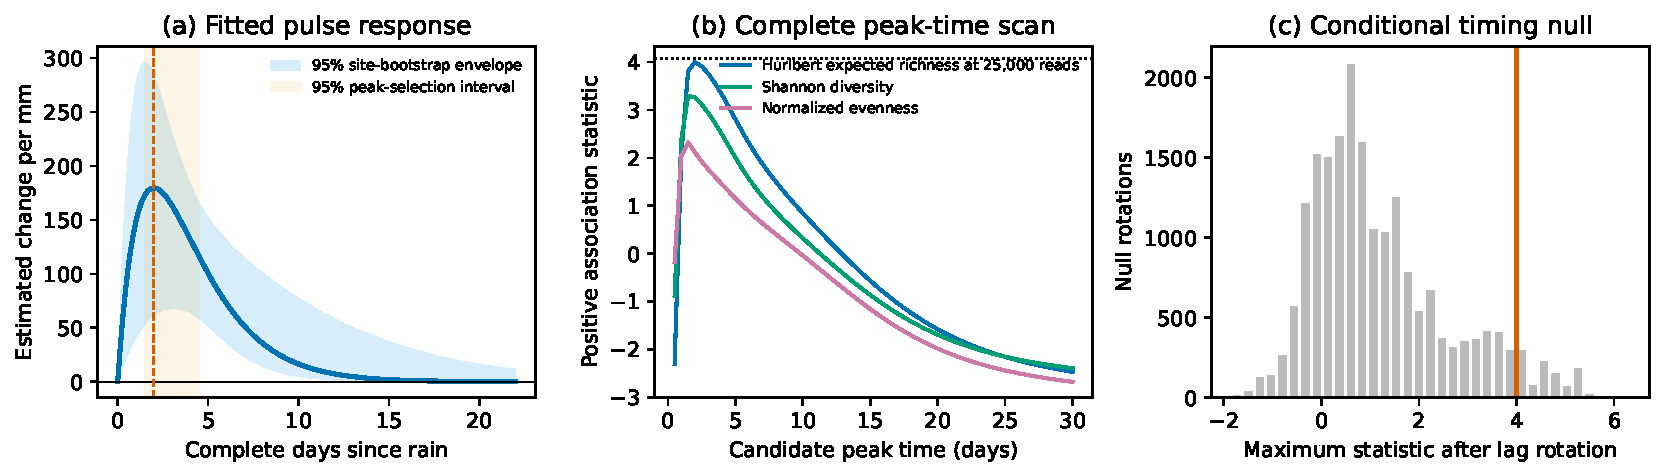
\includegraphics[width=\linewidth]{figures/figS_campaign_rainfall.pdf}
\caption{Fitted antecedent-rain pulse. (a) Estimated change in expected
richness after one millimetre of rain under the selected NASA POWER pulse
kernel. The blue band is the $95\,\%$ site-bootstrap curve envelope, the orange
band is the $95\,\%$ peak-selection interval, and the dashed line marks the
two-day fitted peak. (b) Positive-association
statistics across all candidate peak times for expected richness, Shannon
diversity and normalized evenness; the dotted line is the 95th percentile of
the complete-search null. (c) Conditional null distribution of the largest
positive statistic across all peak times and endpoints under $19{,}999$
within-expedition lag rotations; the red line marks the observed maximum. The
familywise directional probability was $0.056$. The curve estimates an
association, not a causal response or exact biological latency.}
\label{fig:campaign-rainfall-secondary}
\end{figure}

\subsection{Paired PMA endpoints}

For the PMA pairs, Hurlbert expected richness at the minimum common depth of
$123{,}897$ reads was $771.8$ untreated versus $608.5$ treated (exact paired Wilcoxon
$p=0.00781$; eight of nine pairs lower). The mean treated-minus-untreated
difference was $-163.3$ ($95\,\%$ paired-aliquot bootstrap interval
$-274.0$ to $-69.8$). Shannon was $4.19$ versus $4.32$; its mean difference was
$0.130$ ($95\,\%$ interval $-0.154$ to $0.467$; $p=0.652$), so no difference was
detected. Both intervals used $99{,}999$ resamples of the nine matched pairs with
seed $20260805$. The manuscript reports the paired
treatment response only. The surviving protocol record does not preserve the
PMAxx concentration, dark-incubation time, photoactivation duration or
photoactivation device, preventing exact replication of the wet-laboratory
treatment. PMA-seq
is qualitative in complex communities and is affected by matrix, biomass and
taxonomic composition \cite{wang2021pma}. The staged ASV count table supports
re-execution of these endpoints; reproducing it from reads requires separate
public raw-read accessions.

\section{Predicted pathway structure and shotgun encoded function}

\subsection{PICRUSt2 ecology analysis}

PICRUSt2 v2.4.1 predictions matched all $1{,}227$ profiles from the $60$ core
sites. The unstratified input contained $462$ MetaCyc pathways
\cite{metacyc}. Sequencing replicates
were summed within campaign, site and soil position, yielding $633$ grouped
profiles. Of the $462$ pathways, $416$ occurred in at least $20\,\%$ of grouped
profiles. The primary analysis selected the $200$ with the largest mean relative
abundance and applied a $0.5$ pseudocount before CLR transformation. Analyses of
$100$ pathways, all $416$ prevalent pathways and a $1.0$ pseudocount tested the
feature-set and zero-treatment choices.

For geography, campaign-by-position means were removed before profiles were
averaged within each of the $60$ sites. A pre-specified linear and quadratic
transect model accounted for $23.42\,\%$ of predicted pathway composition
($95\,\%$ delete-one-site jackknife interval, $15.46$--$31.39\,\%$;
$p=0.0001$; $9{,}999$ whole-site permutations). Across pathway-set, pseudocount
and leave-one-campaign analyses, the explained share ranged from $21.39$ to
$36.26\,\%$, and every permutation test gave $p=0.0001$.

For soil position, $172$ campaign-by-site blocks contained surface,
shallow-subsurface and root-adjacent profiles. Each complete block was centred
on its own three-position mean and then averaged within site, making the $60$
sites the independent units. The omnibus position statistic was pseudo-$F=6.37$
($p=0.0001$). Standardized paired displacements were $0.453$ for root-adjacent
minus shallow subsurface ($q=0.00015$), $0.429$ for root-adjacent minus surface
($q=0.00015$), and $0.330$ for shallow subsurface minus surface ($q=0.0194$).
The omnibus result and both root-adjacent contrasts passed every pathway-set,
pseudocount and leave-one-campaign test. The shallow-subsurface--surface
contrast did not pass when Trip~$3$ was omitted ($p=0.136$), so it is the weaker
pairwise result.

Pathway-wise sign-flip tests retained the same site-level paired design. One
global correction covered $600$ pathway-by-position tests: $121$ root-adjacent--
shallow, $73$ root-adjacent--surface and $76$ shallow--surface associations passed
$q<0.05$. The supported predictions included amino-acid and cofactor
biosynthesis, carbohydrate degradation and cell-envelope pathways. A separate
family of $200$ pathway--transect correlations retained $92$ pathways. These
follow-up tests identify predicted pathways for direct measurement; because
they are derived from the ASVs, they are not independent evidence of metabolic
activity.

Several supported predictions motivate more specific follow-up experiments.
Along the west--east route, cis-vaccenate biosynthesis, gondoate biosynthesis
and saturated fatty-acid elongation each had $\rho=0.610$--$0.616$
($q\leq3.24\times10^{-6}$), whereas palmitate biosynthesis had
$\rho=-0.527$ ($q=1.18\times10^{-4}$). Root-adjacent soil exceeded both
bulk-soil positions for predicted glucose and xylose degradation, fructuronate
and $4$-aminobutanoate degradation, polyamine biosynthesis and thiamin
diphosphate biosynthesis (all $q\leq0.0162$). These are pathway predictions,
not measurements of membrane adaptation, plant-derived substrate use or
metabolite exchange. The selected MetaCyc set did not contain a dedicated
UV-repair pathway. Testing UV protection or DNA repair therefore requires a
pre-specified gene-level analysis rather than an interpretation added to this
pathway screen. The complete $600$ position tests and $200$ geographic tests are
in \path{analysis/v3/picrust2_ecology/}.

Weighted NSTI had median $0.1648$ across the $1{,}227$ profiles (range
$0.0053--0.7819$). The median was $0.2011$ in shallow-subsurface, $0.1681$ in surface
and $0.1340$ in root-adjacent profiles. Lower NSTI means that the contributing
ASVs are closer to the reference genomes used for prediction. Exact grouped
cohorts, primary and sensitivity tests, pathway-level results, NSTI summaries,
seeds and checksums are archived under
\path{analysis/v3/picrust2_ecology/}.

\subsection{Resolution-matched shotgun encoded-function test}

Table~\ref{tab:shotgun-revised} reports the resolution-matched functional
turnover test and its intact-genome-label null.

\begin{table}[H]\centering\scriptsize
\caption{Resolution-matched encoded-function null. ``Encoded'' is the median
Bray--Curtis dissimilarity of abundance-weighted KO profiles; the null
reassigns intact genome annotation profiles among fixed genome-abundance
vectors ($999$ permutations). $p_{\rm L}$ and $p_{\rm U}$ are the
plus-one-corrected lower- and upper-tail values.}
\label{tab:shotgun-revised}
\resizebox{\textwidth}{!}{%
\begin{tabular}{llrrrrlrr}
\toprule
Annotation basis & Group & $n$ & Taxonomic & Encoded &
Encoded/taxonomic & Null median [$95\,\%$ interval] & $p_{\rm L}$ & $p_{\rm U}$ \\
\midrule
KO copy count & All & $150$ & $0.82272$ & $0.13386$ & $0.16271$ &
$0.08733$ [$0.08459$, $0.09067$] & $1.000$ & $0.001$ \\
 & Shallow subsurface & $44$ & $0.80929$ & $0.13270$ & $0.16397$ &
$0.08400$ [$0.08029$, $0.08838$] & $1.000$ & $0.001$ \\
 & Root-adjacent & $79$ & $0.81810$ & $0.13348$ & $0.16316$ &
$0.08889$ [$0.08567$, $0.09269$] & $1.000$ & $0.001$ \\
 & Surface & $27$ & $0.75209$ & $0.11254$ & $0.14964$ &
$0.08138$ [$0.07595$, $0.08765$] & $1.000$ & $0.001$ \\
\addlinespace
Within-genome relative & All & $150$ & $0.82272$ & $0.13659$ & $0.16602$ &
$0.08882$ [$0.08592$, $0.09315$] & $1.000$ & $0.001$ \\
 & Shallow subsurface & $44$ & $0.80929$ & $0.13615$ & $0.16824$ &
$0.08544$ [$0.08165$, $0.09040$] & $1.000$ & $0.001$ \\
 & Root-adjacent & $79$ & $0.81810$ & $0.13418$ & $0.16402$ &
$0.09041$ [$0.08702$, $0.09523$] & $1.000$ & $0.001$ \\
 & Surface & $27$ & $0.75209$ & $0.11573$ & $0.15388$ &
$0.08284$ [$0.07758$, $0.09023$] & $1.000$ & $0.001$ \\
\bottomrule
\end{tabular}
}
\end{table}

The staged, checksum-tracked CoverM and eggNOG-derived inputs support
re-execution of the following downstream test; they do not support regeneration
from raw reads without the separate MAG catalogue and upstream metadata. The
observed encoded-functional dissimilarity was greater, not smaller, than
the complete $95\,\%$ null interval under both annotation bases and in every
compartment. Accordingly, encoded-functional turnover was lower than
taxonomic turnover in absolute terms, but higher than the
resolution-matched genome-label null.
Functional convergence or redundancy beyond feature resolution is not
supported. Observed turnover exceeded every null replicate
($p_{\rm U}=0.001$), but this test does not identify a mechanism. The null preserves the
genome-abundance matrix, every intact annotation profile and KO prevalence;
it is not a metabolic-network null. Only $0.28465$ of the CoverM total was
assigned to the annotated $990$-genome set on average. The result therefore
concerns genome-resolved encoded potential in a minority fraction, not
direct-read function, expression, activity or flux.

A top-$K$ sensitivity retained $1{,}000$, $2{,}000$ or $5{,}000$ KOs. Observed median
KO-copy Bray--Curtis dissimilarity was $0.1005$, $0.1339$ and $0.1721$, compared
with label-null medians of $0.0670$, $0.0873$ and $0.1174$, respectively.
Observed turnover exceeded the null upper interval in all three configurations
($p_{\rm U}=0.001$ throughout), so the conclusion does not depend on the
primary $K=2{,}000$ choice.

Across $125$ samples and $3{,}471$ shared KOs, the PICRUSt2--shotgun whole-profile
Spearman correlation had median $0.743$ ($95\,\%$ whole-site bootstrap interval
$0.731--0.751$) and community-mean $0.806$ ($0.793--0.812$). The $9{,}999$ bootstrap
samples kept all matched profiles from the same field site together and used
seed $20260805$. Rare-marker
agreement is much weaker and not distinguishable from zero (RuBisCO
$r=0.16$, two-sided $p=0.067$), so the whole-profile association
is not treated as rare-marker validation. These predictions used separately
executed Trips~$1--4$ and Trip~$5$ input sets containing $330{,}830$ ASVs, rather than
the $351{,}472$-ASV combined canonical table used for the primary ecological
analyses.

The staged positive-only metabolic-marker table contains $132$ genome records annotated with both
RuBisCO and phosphoribulokinase. The complete upstream screened-genome
manifest was not preserved in the local analysis bundle, so no denominator or
genome fraction is reported. This supports candidate Calvin-cycle genomic
potential in the recovered output. The supplied pathway screen contains no
positive calls for rTCA, Wood--Ljungdahl or the $3$-HP cycle. It contains $33$
single-marker hits for the hydroxybutyrate cycle; the latter marker is not
pathway-specific, and zero calls are not evidence of biological absence. The
result does not exclude phototrophy,
show carbon fixation or identify an energy source. Hydrogenase and
CO-dehydrogenase product labels are not sufficient to establish high-affinity
atmospheric oxidation; \emph{mcrA} and \emph{nifH} non-detections are bounded
by recovery and annotation sensitivity. No profile-HMM, catalytic-motif,
phylogenetic, synteny or direct-read confirmation was included, so no
trace-gas pathway or activity claim is made.

\section{Cross-desert and regional context}

\subsection{Quantitative comparison with public Atacama surveys}

We compared effects rather than merging feature tables because the surveys
used different $16$S regions, reference databases and sampling designs. The
Atacama aridity-gradient input is an archived site-level table derived from
QIITA study $10360$. The upstream V4 OTU profiles were rarefied $100$ times to
$12{,}000$ reads and technical replicates were averaged within site. The replayed
analysis retained $16$ sites with complete soil relative humidity and spatial
information. Soil relative humidity was positively associated with Shannon
diversity ($\rho=0.8904$, $p=3.80\times10^{-6}$). The association remained
after ranked humidity and diversity were adjusted for latitude, longitude and
elevation (partial $\rho=0.6753$, $p=0.00409$). Rarefied richness gave the same
direction (raw $\rho=0.8712$; partial $\rho=0.6445$).

For the Atacama pit, all $62$ reprocessed intracellular-DNA profiles exceeded
$8{,}000$ reads. Replicates represented $23$ sampled depths from $2.5$ to $420$~cm. We
combined replicate counts within depth, retained the $200$ leading genera and
tested three zones in CLR coordinates. Composition differed among zones
(pseudo-$F=1.463$, $p=0.0014$, $9{,}999$ label permutations). After $100$
rarefactions per profile and averaging within depth, richness increased only
weakly with depth ($\rho=0.381$, $p=0.0725$), and Shannon diversity had no
monotonic trend ($\rho=0.120$, $p=0.587$). The compositional result supports
depth as a recurring source of habitat structure; the diversity direction is
not portable from one depth design to another.

These comparisons do not identify a common cause. Soil relative humidity in
the Atacama and a $49$-month atmospheric humidity mean in the Empty Quarter are
different exposures. The Atacama pit is one vertical profile sampled to
$4.2$~m, whereas Empty Quarter positions span only $0--10$~cm and include loose
root-adjacent soil. Exact inputs, parameters, software versions and checksums
are recorded under \path{analysis/v3/cross_desert_context/}. The archived
Atacama-gradient table reproduces the site-level tests, but regeneration of
that table from the original QIITA BIOM file remains an upstream step.

\subsection{Design boundaries in related studies}

Table~\ref{tab:sota} places the survey against regional observational and
experimental precedents while retaining their design boundaries.

{\footnotesize
\begin{longtable}{P{3.0cm}P{4.6cm}P{5.6cm}}
\caption{Studies that define the comparison and evidential boundary.}\label{tab:sota}\\
\toprule
Study & Design & Relevance to this manuscript \\
\midrule
\endfirsthead
\toprule
Study & Design & Relevance to this manuscript \\
\midrule
\endhead
McKay et al.\ $2016$, ``An Unusual Inverted Saline Microbial Mat Community in
an Interdune Sabkha in the Rub' al Khali'' \cite{mckay2016sabkha} & One groundwater-fed Liwa sabkha,
UAE; salt mat microbiology and geochemistry & Direct Rub' al-Khali precedent,
but a specialized saline mat rather than open Saudi landscape soils \\
Yasir et al.\ $2015$, ``Composition of soil microbiome along elevation gradients
in southwestern highlands of Saudi Arabia'' \cite{yasir2015elevation} & Ten soils across four
southwestern highland elevations; $16$S V6 pyrosequencing and soil chemistry &
Early Saudi spatial soil-microbiome precedent; a small highland gradient rather
than a repeated hyperarid transect \\
Aslam et al.\ $2016$, ``Soil compartment is a major determinant of the impact of
simulated rainfall on desert microbiota'' \cite{aslam2016rainfall} & In-situ watering of Saudi desert
crust, root-attached and broader root-zone soil & Direct experimental
compartment/rainfall comparator; shows why our five observational dates cannot
substitute for a manipulated response trajectory \\
Eida et al.\ $2018$, ``Desert plant bacteria reveal host influence and beneficial
plant growth properties'' \cite{eida2018desertplants} & Barren soil, rhizosphere and root endosphere of
identified hosts in Jizan and Al Wahbah & Defines the sampling and host
metadata needed for rhizosphere/endosphere and host-filter claims \\
Khan and Khan $2020$, ``Microbial communities and their predictive functional
profiles in the arid soil of Saudi Arabia'' \cite{khan2020saudi} & Abha, Hafar Al Batin and
Muzahmiya; $16$S and PICRUSt; includes rhizosphere & Direct Saudi arid-soil
precedent; prevents a ``first Saudi survey'' claim \\
Maurice et al.\ $2023$, ``Fertility islands, keys to the establishment of plant
and microbial diversity in a highly alkaline hot desert'' \cite{maurice2023fertility} & AlUla vegetation
patches, soils, geochemistry and microbial diversity & Saudi fertility-island
and plant-associated geochemistry comparator; unlike operationally defined
root-adjacent soil \\
Maurice et al.\ $2024$, ``Networking the desert plant microbiome''
\cite{maurice2024alula} & Roots and
rhizospheres of six identified plant species in AlUla, Saudi Arabia &
Shows the host and root metadata needed for a plant-selective-filter
mechanism \\
Jalal et al.\ $2022$, Saudi coastal halophyte compartments
\cite{jalal2022saudi} &
Southern Corniche halophyte-associated soil, rhizosphere, root and leaf
endosphere samples & Saudi saline-soil precedent; a specialized host system
that does not validate salinity physiology in our XRF gradient \\
Mousa et al.\ $2024$, ``High-throughput sequencing reveals the structure and
metabolic resilience of desert microbiome confronting climate change''
\cite{mousa2024arabian} &
Rhizosphere and endosphere sequencing of native Arabian desert plants in
Dubai and Al Ain, UAE & UAE/Arabian plant-desert comparator; distinct from the open-soil
landscape design used here \\
Pan et al.\ $2022$, ``Aridity Threshold Induces Abrupt Change of Soil Abundant
and Rare Bacterial Biogeography'' \cite{pan2022aridity} & Chinese dryland gradient spanning aridity
threshold; abundant/rare assembly & Hypothesis-level comparison; our
one-dimensional transect cannot identify an aridity response \\
Bay et al.\ $2020$, Negev soil biogeography \cite{bay2020negev} & $99$ soils
across as much as $189$~km; fine-resolution community turnover and distance
decay & Independent hot-desert support for spatial turnover; primer, distance
metric and landscape differ, so coefficients are not directly comparable \\
Ronca et al.\ $2015$, Namib dune/interdune transects
\cite{ronca2015namib} & Surface soils across repeated dune and interdune
habitats & Shows habitat-specific turnover in another sand desert; it does not
provide the repeated, three-position design used here \\
Pombubpa et al.\ $2020$, Mojave biocrust survey
\cite{pombubpa2020mojave} & $48$ surface and subsurface profiles across four
sites and crust types & Independent support for depth-related composition;
biocrust and open-sand positions are different habitats \\
Demergasso et al.\ $2023$, ``Hyperarid soil microbial community response to
simulated rainfall'' \cite{demergasso2023rainfall} & Controlled, replicated $30$-day rainfall treatment &
Shows the trajectory and controls needed to establish bloom/relaxation \\
Horstmann et al.\ $2024$, ``Persistent microbial communities in hyperarid
subsurface habitats of the Atacama Desert'' \cite{horstmann2024atacama} & Depth profile to $4.2$~m;
intracellular DNA & Appropriate subsurface comparison; our $5--10$~cm samples do
not show a deep refugium or activity \\
El Moatassem et al.\ $2025$, ``Soil salinity hazard monitoring with portable
X-ray fluorescence spectrometry and electrical conductivity meters''
\cite{elmoatassem2025pxrf} & pXRF
models calibrated against EC & Establishes the independent validation required
before calling the XRF axis salinity \\
Tribbia et al.\ $2026$, ``Trace gas oxidation supports sub-surface microbial
communities across Namib Desert fog and aridity gradients''
\cite{tribbia2026tracegas} & Gas uptake,
wetting, ATP, respiration, abundance and geochemistry & Defines the direct
activity evidence missing from our marker inventory \\
\bottomrule
\end{longtable}
}

This study is a large, repeated landscape survey of open sand, shallow
subsurface and root-adjacent Saudi Rub' al-Khali soils,
joined to distinct field/laboratory XRF products and an analysis-ready shotgun
subset. It is not
the first Saudi arid-soil study, first Rub' al-Khali microbial study, proof of
a seasonal bloom, or evidence of active atmospheric chemosynthesis.

\section{Uncertainty estimates for headline results}

Table~\ref{tab:headline-uncertainty} lists the point estimates that carry the
main ecological interpretation. Brackets are $95\,\%$ sampling intervals unless
they are identified as a sensitivity range or interquartile range. These
quantities answer different questions. Sampling intervals describe variation
among sites or matched pairs. Rain peak-selection intervals include the choice
among candidate peak times but remain conditional on one rainfall product and
the fitted nuisance adjustment. The pH influence and XRF model ranges describe
specific analysis choices and are not confidence intervals. The contamination
interquartile range describes variation among linked profiles, not uncertainty
in the median.

For paired contrasts and correlations, bootstrap resampling kept repeated
observations from one site or aliquot pair together. For geographic $R^2$,
distance slopes and replacement shares, the delete-one-site jackknife removed
the complete site; for pairwise distances it also removed every pair involving
that site. Functional-profile bootstraps kept all profiles from a field site
together. Exact machine-readable values, method labels, independent units and
source files are in
\path{analysis/v3/headline_uncertainty/headline_uncertainty.tsv}.

\begingroup
\scriptsize
\begin{longtable}{P{6.3cm}P{3.3cm}P{5.2cm}}
\caption{Headline estimates and quantified uncertainty. Bootstrap intervals
are percentile intervals. CI denotes a $95\,\%$ confidence interval.}
\label{tab:headline-uncertainty}\\
\toprule
Estimand & Estimate [interval or range] & Basis and independent unit \\
\midrule
\endfirsthead
\multicolumn{3}{l}{\tablename\ \thetable\ continued}\\[2pt]
\toprule
Estimand & Estimate [interval or range] & Basis and independent unit \\
\midrule
\endhead
\midrule
\multicolumn{3}{r}{Continued on the next page}\\
\endfoot
\bottomrule
\endlastfoot
\multicolumn{3}{l}{\textbf{Geography}} \\
Quadratic transect partial $R^2$ & $0.402$ [$0.325$,$0.478$] & Site-jackknife CI; $60$ sites \\
Aitchison slope per $100$~km, surface & $1.351$ [$0.905$,$1.796$] & Site-jackknife CI; $60$ sites \\
Aitchison slope per $100$~km, shallow subsurface & $1.510$ [$1.092$,$1.929$] & Site-jackknife CI; $60$ sites \\
Aitchison slope per $100$~km, root-adjacent & $1.180$ [$0.698$,$1.662$] & Site-jackknife CI; $60$ sites \\
Replacement share, surface & $0.715$ [$0.636$,$0.793$] & Site-jackknife CI; $60$ sites \\
Replacement share, shallow subsurface & $0.692$ [$0.607$,$0.776$] & Site-jackknife CI; $60$ sites \\
Replacement share, root-adjacent & $0.747$ [$0.676$,$0.818$] & Site-jackknife CI; $60$ sites \\
\addlinespace
\multicolumn{3}{l}{\textbf{Soil position}} \\
Standardized composition, shallow minus surface & $0.331$ [$0.306$,$0.404$] & Paired-site bootstrap; $60$ sites \\
Standardized composition, root-adjacent minus surface & $0.433$ [$0.386$,$0.509$] & Paired-site bootstrap; $60$ sites \\
Standardized composition, root-adjacent minus shallow & $0.478$ [$0.423$,$0.556$] & Paired-site bootstrap; $60$ sites \\
Mean Shannon difference, shallow minus surface & $0.075$ [$-0.089$,$0.235$] & Paired-site bootstrap; $60$ sites \\
Mean Shannon difference, root-adjacent minus surface & $-0.130$ [$-0.321$,$0.079$] & Paired-site bootstrap; $60$ sites \\
Mean Shannon difference, root-adjacent minus shallow & $-0.206$ [$-0.398$,$-0.001$] & Paired-site bootstrap; $60$ sites \\
Mean evenness difference, shallow minus surface & $0.0125$ [$0.0008$,$0.0251$] & Paired-site bootstrap; $60$ sites \\
Mean evenness difference, root-adjacent minus surface & $-0.0315$ [$-0.0448$,$-0.0186$] & Paired-site bootstrap; $60$ sites \\
Mean evenness difference, root-adjacent minus shallow & $-0.0440$ [$-0.0572$,$-0.0313$] & Paired-site bootstrap; $60$ sites \\
\addlinespace
\multicolumn{3}{l}{\textbf{Long-term climate}} \\
Temperature versus Shannon, Spearman $\rho$ & $-0.711$ [$-0.833$,$-0.520$] & Paired-site bootstrap; $60$ sites \\
Temperature versus expected richness, $\rho$ & $-0.795$ [$-0.887$,$-0.639$] & Paired-site bootstrap; $60$ sites \\
Temperature versus evenness, $\rho$ & $-0.584$ [$-0.753$,$-0.359$] & Paired-site bootstrap; $60$ sites \\
Monthly rain versus Shannon, $\rho$ & $-0.470$ [$-0.671$,$-0.211$] & Paired-site bootstrap; $60$ sites \\
Monthly rain versus expected richness, $\rho$ & $-0.495$ [$-0.702$,$-0.226$] & Paired-site bootstrap; $60$ sites \\
Monthly rain versus evenness, $\rho$ & $-0.298$ [$-0.532$,$-0.023$] & Paired-site bootstrap; $60$ sites \\
Humidity versus Shannon, $\rho$ & $-0.701$ [$-0.834$,$-0.490$] & Paired-site bootstrap; $60$ sites \\
Humidity versus expected richness, $\rho$ & $-0.770$ [$-0.877$,$-0.593$] & Paired-site bootstrap; $60$ sites \\
Humidity versus evenness, $\rho$ & $-0.522$ [$-0.713$,$-0.266$] & Paired-site bootstrap; $60$ sites \\
\addlinespace
\multicolumn{3}{l}{\textbf{pH and elemental composition}} \\
Geographic partial $R^2$ before pH adjustment & $0.358$ [$0.358$,$0.362$] & Prespecified influence range; not a CI \\
Geographic partial $R^2$ after pH adjustment & $0.196$ [$0.187$,$0.196$] & Prespecified influence range; not a CI \\
pH transect partial $R^2$ & $0.846$ [$0.826$,$0.846$] & Prespecified influence range; not a CI \\
Elemental-axis partial $R^2$ & $0.00358$ [$0.00311$,$0.00543$] & Prespecified model range; not a CI \\
\addlinespace
\multicolumn{3}{l}{\textbf{Recent rain}} \\
NASA POWER richness change per mm at peak & $179.6$ [$92.1$,$267.1$] & Site-clustered sandwich CI; $60$ sites \\
NASA POWER partial $R^2$ at peak & $0.0364$ [$0.0060$,$0.0787$] & Fixed-curve site bootstrap; $60$ sites \\
NASA POWER selected peak, complete days & $2.0$ [$1.5$,$4.5$] & Peak-selection site bootstrap; $60$ sites \\
Open-Meteo richness change per mm at peak & $327.5$ [$141.1$,$514.0$] & Site-clustered sandwich CI; $60$ sites \\
Open-Meteo partial $R^2$ at peak & $0.0384$ [$0.0057$,$0.0899$] & Fixed-curve site bootstrap; $60$ sites \\
Open-Meteo selected peak, complete days & $1.0$ [$0.5$,$6.5$] & Peak-selection site bootstrap; $60$ sites \\
\addlinespace
\multicolumn{3}{l}{\textbf{Predicted function}} \\
PICRUSt2 pathway transect $R^2$ & $0.234$ [$0.155$,$0.314$] & Site-jackknife CI; $60$ sites \\
PICRUSt2 position, shallow minus surface & $0.330$ [$0.296$,$0.501$] & Paired-site bootstrap; $60$ sites \\
PICRUSt2 position, root-adjacent minus surface & $0.429$ [$0.350$,$0.566$] & Paired-site bootstrap; $60$ sites \\
PICRUSt2 position, root-adjacent minus shallow & $0.453$ [$0.412$,$0.549$] & Paired-site bootstrap; $60$ sites \\
Median within-sample PICRUSt2--shotgun $\rho$ & $0.743$ [$0.731$,$0.751$] & Whole-site bootstrap; $125$ profiles \\
Community-mean PICRUSt2--shotgun $\rho$ & $0.806$ [$0.793$,$0.812$] & Whole-site bootstrap; $125$ profiles \\
\addlinespace
\multicolumn{3}{l}{\textbf{Assay controls}} \\
PMA richness difference, treated minus untreated & $-163.3$ [$-274.0$,$-69.8$] & Paired-aliquot bootstrap; nine pairs \\
PMA Shannon difference, treated minus untreated & $0.130$ [$-0.154$,$0.467$] & Paired-aliquot bootstrap; nine pairs \\
Candidate-read fraction per linked profile & $0.00403$ [$0.00155$,$0.00987$] & Empirical median [IQR]; $217$ profiles \\
\end{longtable}
\endgroup

\bibliographystyle{plain}
\bibliography{sample}

\end{document}
